
\documentclass[fleqn,addpoints]{exam}

\usepackage{graphicx}
\usepackage{float}
\usepackage{amsmath}
\usepackage{cancel}
\usepackage{polynom}
\usepackage{caption}

\printanswers

\ifprintanswers 
\usepackage{2in1, lscape} 
\fi

\title{Math 115 Homework 15}
\date{March 15, 2011}

\begin{document}

\maketitle

% \begin{figure}[H]
%   \centering
%   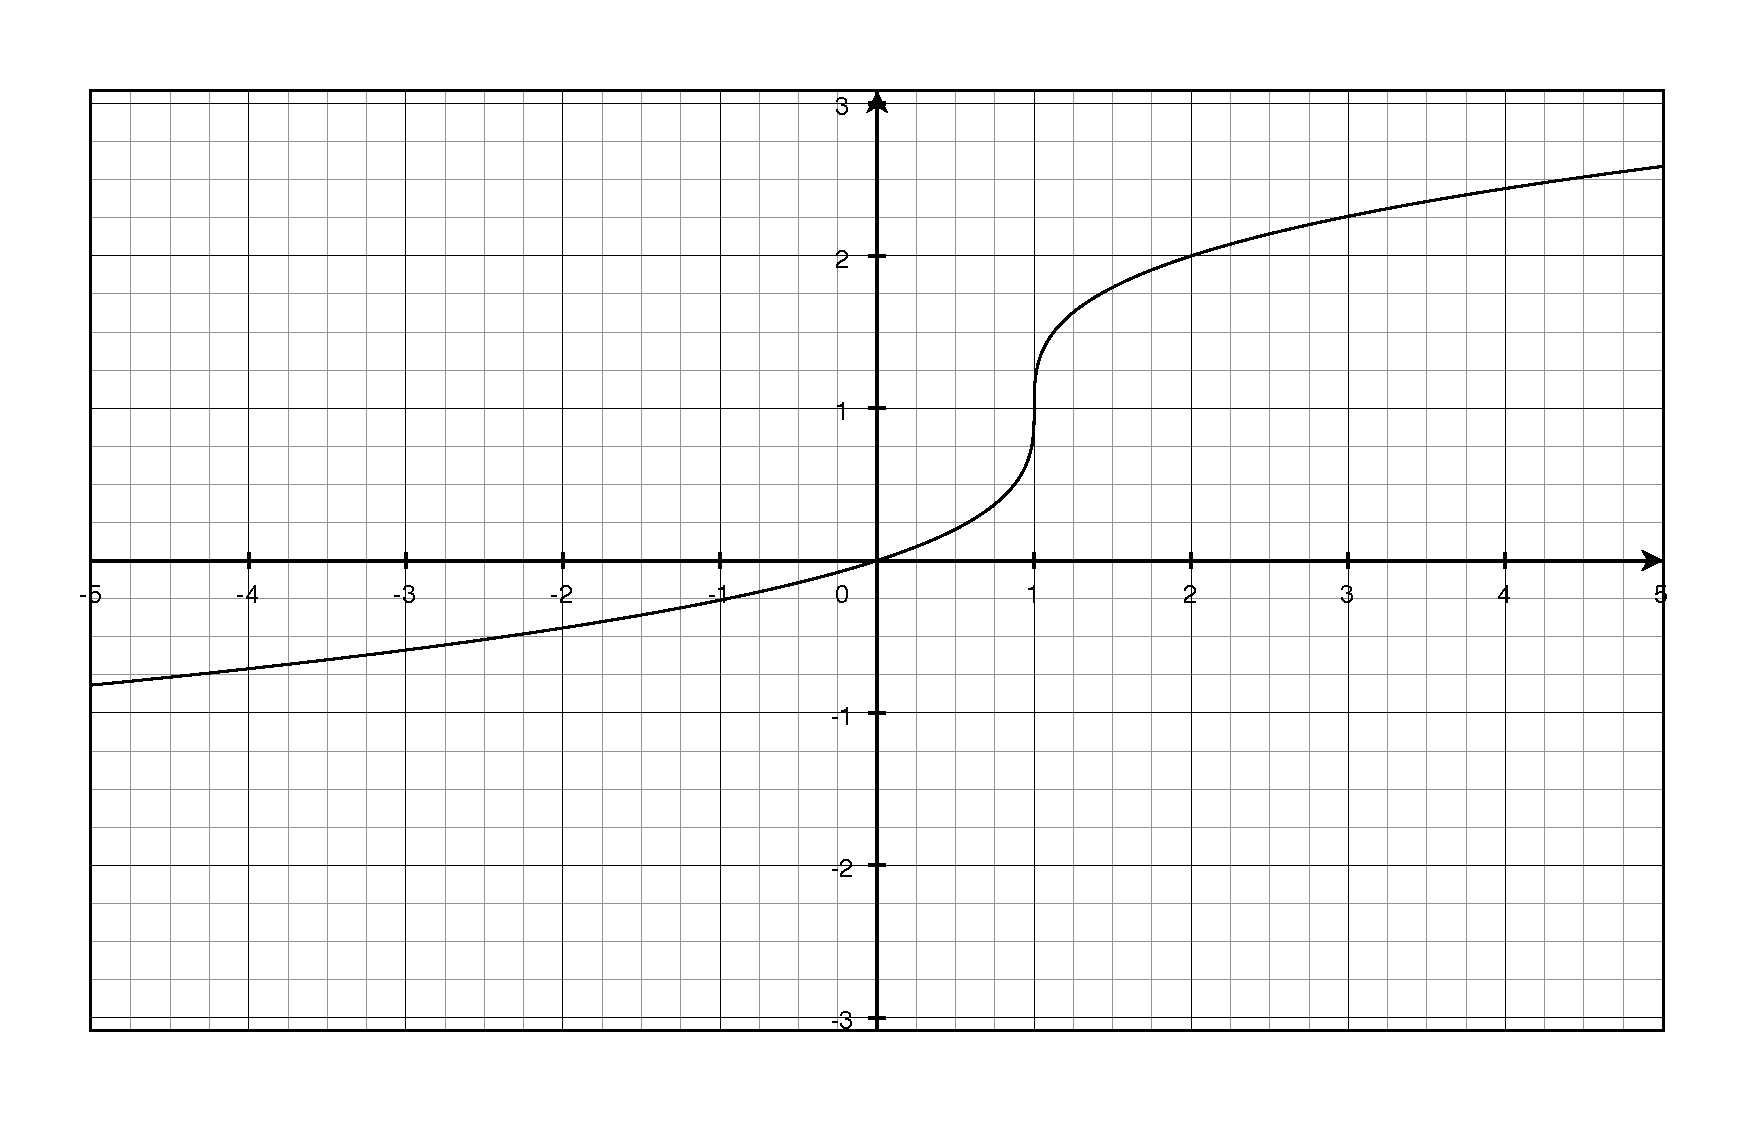
\includegraphics[scale=.3]{question7.eps}
%   \caption*{Question 7}
% \end{figure}

\section{Homework}

Some of the problems require a calculator with {\em log} and {\em ln} operations.  None of them require a graphing
calculator.  If you don't have a calculator, you can borrow one of the UBB ones when you are in the PAB.

Larson/Hostetler:

\begin{itemize}
  \item pp 296-299: 11-14, 27-28, 56, 64, 72
  \item pp 307-310: 1-5, 11-15, 19-24, 45-50, 51, 54, 69, 76
\end{itemize}


\section{Extra Credit}

March Madness is upon us.  And, of course, the first thing most people think of when they think about March Madness is math.

Suppose you have basketball tournament with $n$ teams.  In each round, every team plays one game and the losing teams
are eliminated.  Of course depending on $n$, there may be a round where not every team plays (for instance, the 
``play in'' round of March Madness only features eight teams).

Find a function $f(n)$ which gives the number of games the champion will have to win in a tournament with $n$ teams.

\begin{solution}

If you work backwards from the final round, the final round has 2 teams, the semi-final has 4 teams (Final Four), the
previous round has 8 teams (Elite Eight), and so on.  So, counting the final as round 1, there are $2^r$ teams in
round $r$.

A tournament with $2^r$ teams has $r$ rounds and you need to win a game in each round, so you need to win $r$ games in a 
tournament with $2^r$ teams.

You can say this in two different ways:
\begin{align*}
  number\_of\_teams &= 2^{number\_of\_rounds} \\
  number\_of\_rounds &= \log_2 number\_of\_teams \\
\end{align*}

The only complication is when the number of teams isn't a power of two.  In this case, there is a ``play in'' round
which eliminates enough teams to get the remaining number down to a power of two.  In the NCAA basketball tournament,
there are 68 teams originally and 8 of them have to play one extra round.

\end{solution}

\ifprintanswers

\section{Pages 296-299}

\begin{description}

\item[11] d
\item[12] c
\item[13] a
\item[14] b

\item[27]
\begin{figure}[H]
  \centering
  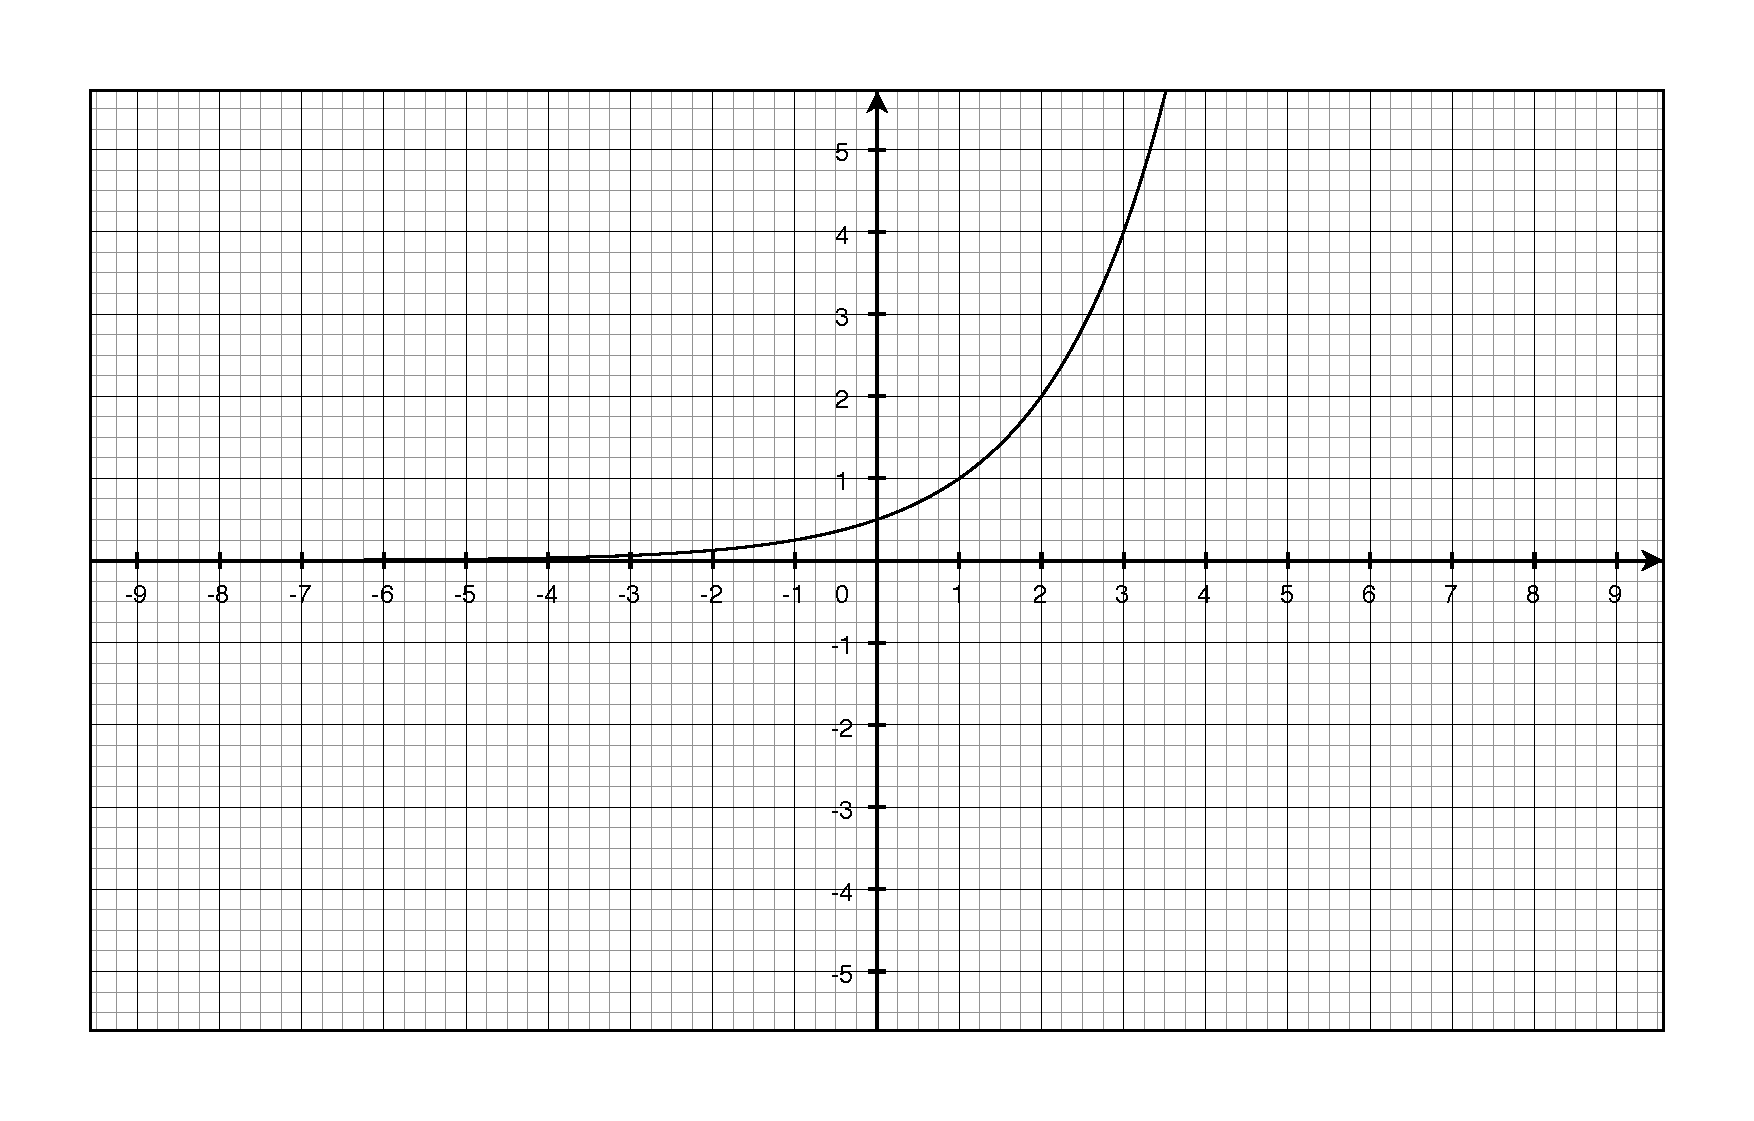
\includegraphics[scale=.3]{question27.eps}
  \caption*{Question 27: $f(x) = 2^{x-1}$}
\end{figure}

\item[28]
\begin{figure}[H]
  \centering
  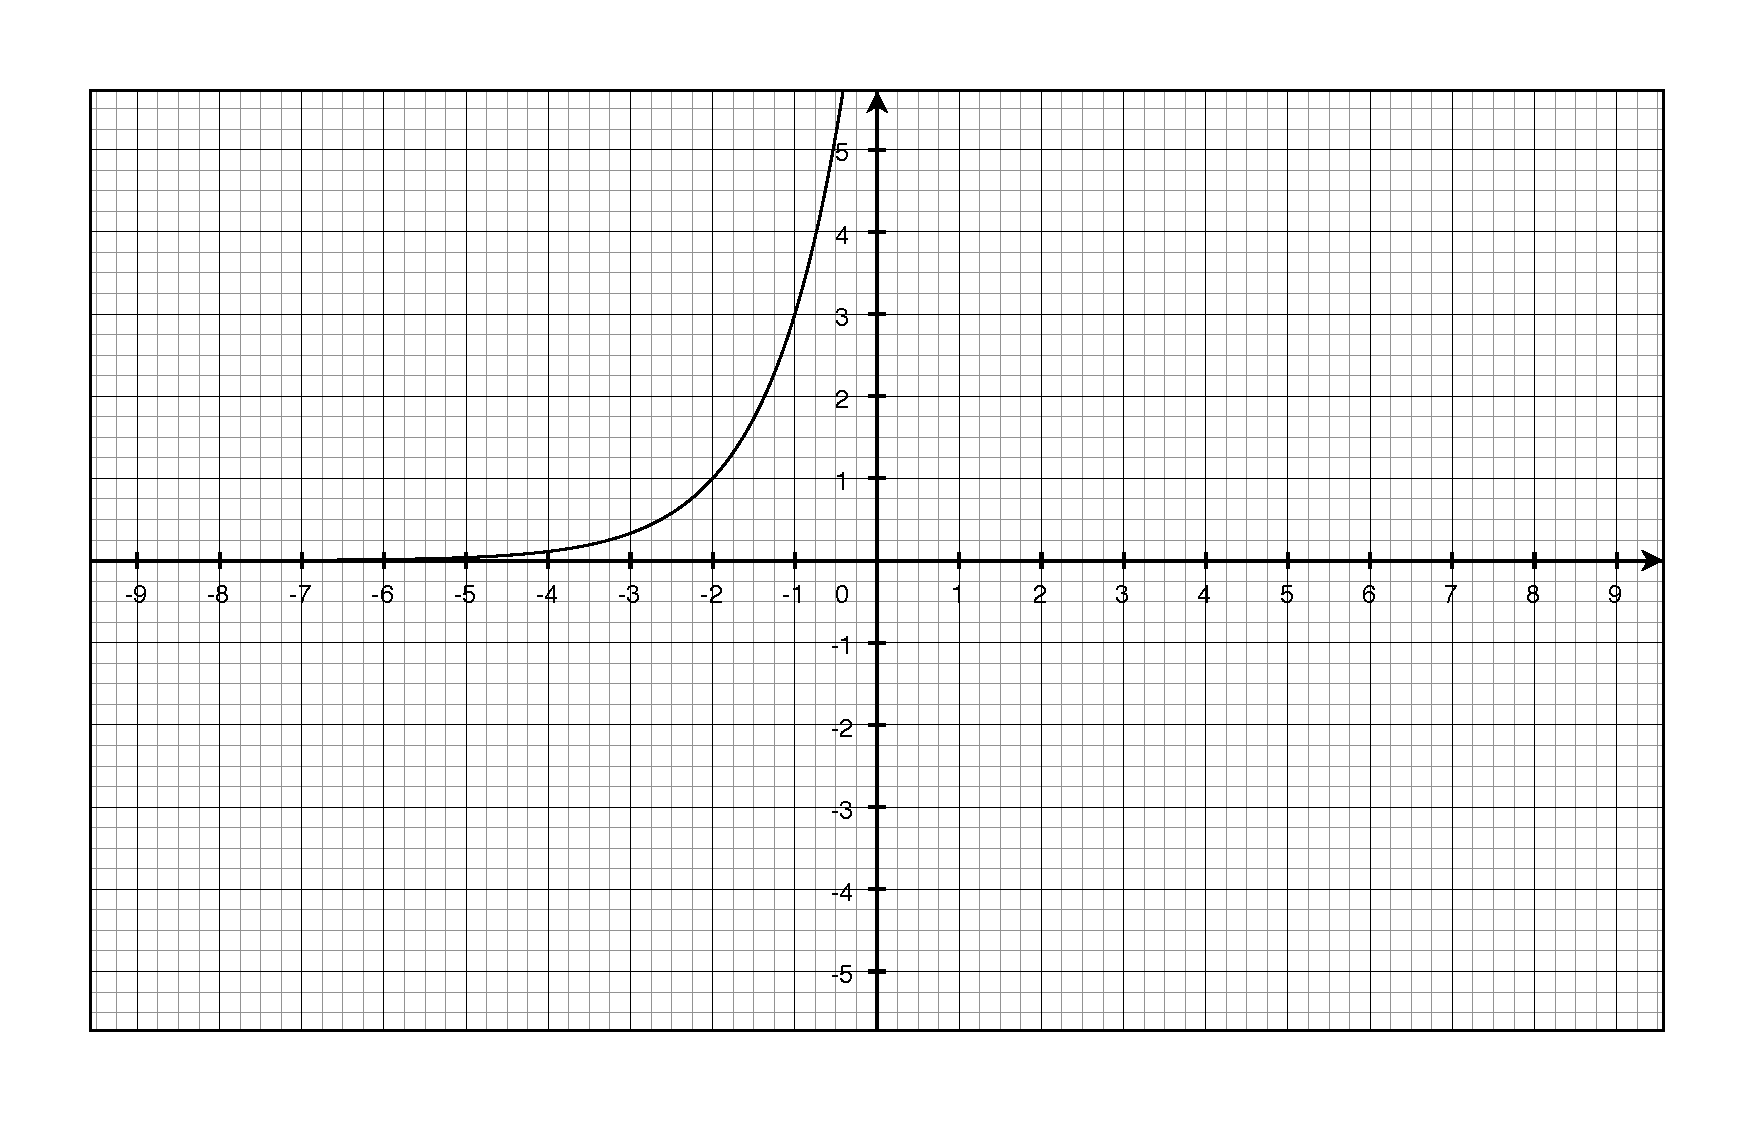
\includegraphics[scale=.3]{question28.eps}
  \caption*{Question 28: $f(x) = 3^{x+2}$}
\end{figure}

\item[56]
\begin{tabular}{|c||c|c|c|c|c|c|}
\hline
n & 1 & 2 & 4 & 12 & 365 & Continuous \\
\hline 
A & \$1,790.85 & \$1,806.11 & \$1,814.02 & \$1,819.40 & \$1,822.03 & \$1,822.12 \\
\hline 
\end{tabular}

\item[64]

Using $A=Pe^{rt}$, $A = 5000 \cdot e^{.075 \cdot 50} = 212,605.41$

\item[72]

\begin{description}

\item[a]
\[
Q(0) = 10
\]

\item[b]
\[
  Q(2000) = 10 \left( \frac{1}{2} \right)^{2000/5730} = 7.85
\]

\item[c]
\begin{figure}[H]
  \centering
  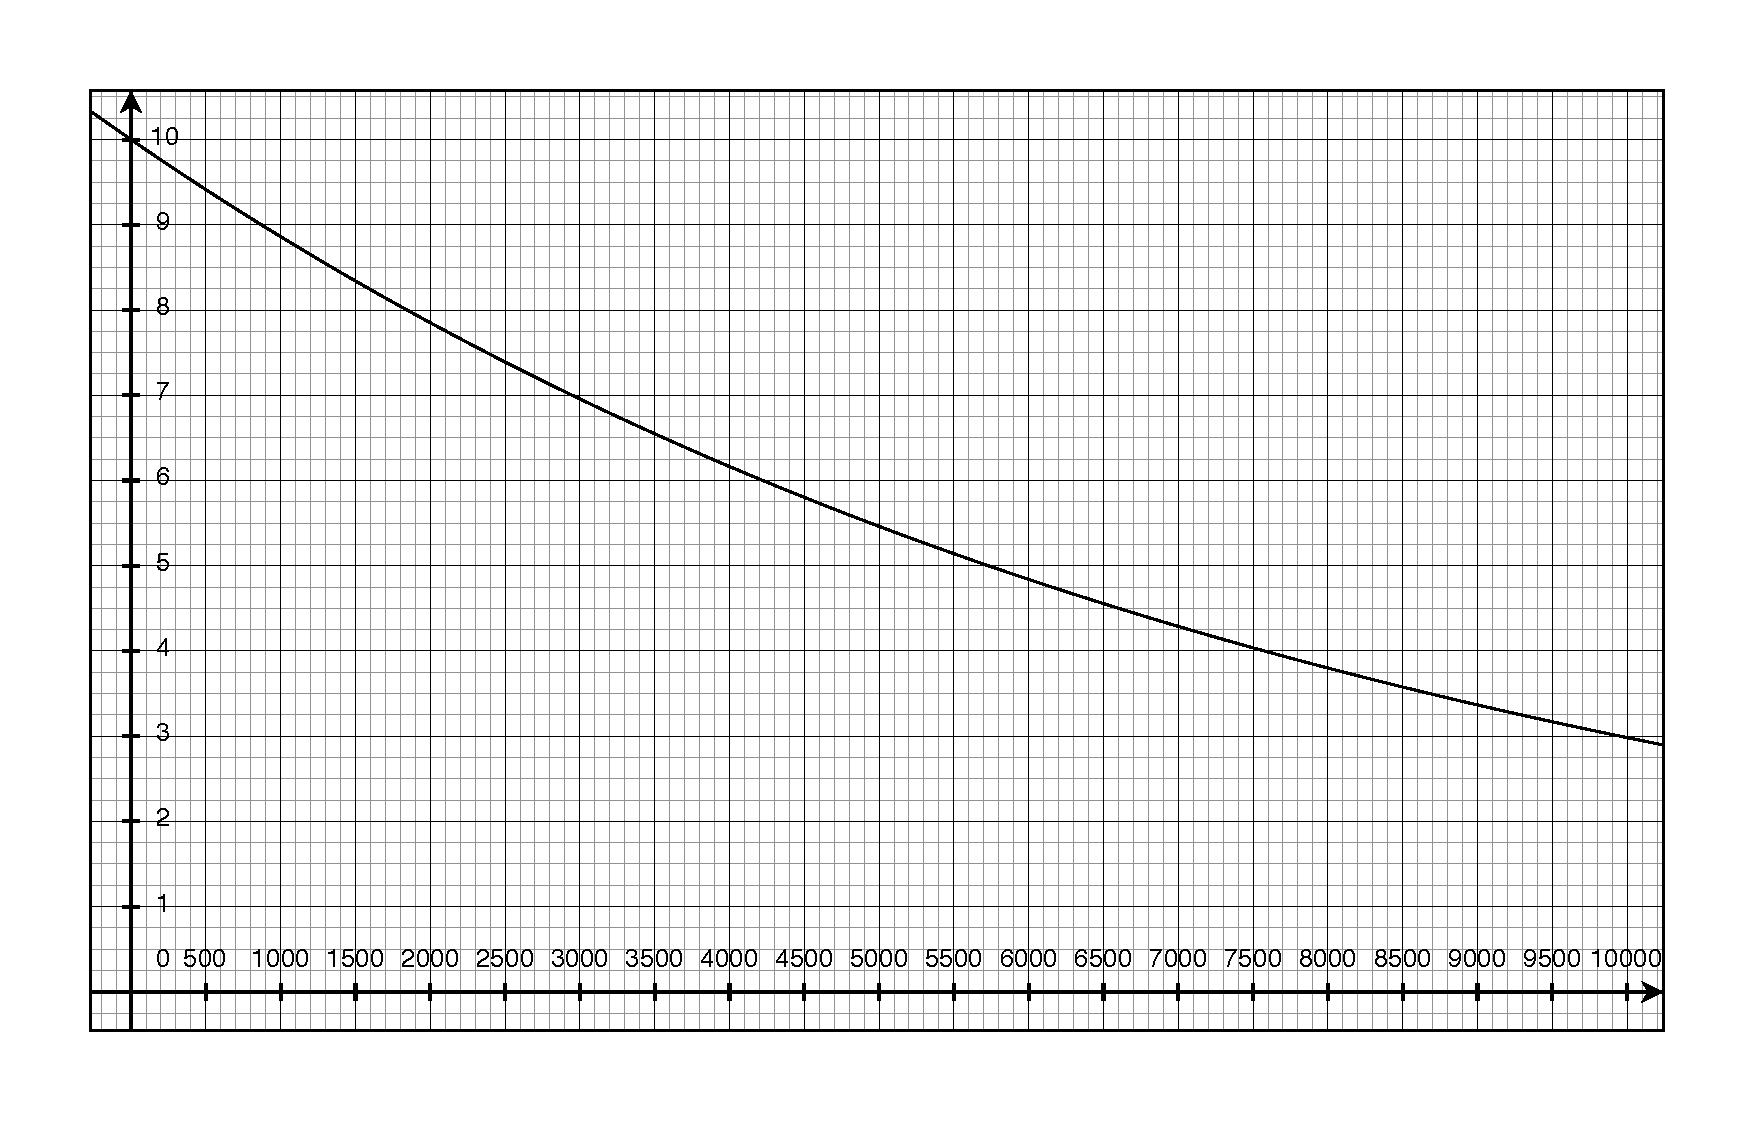
\includegraphics[scale=.3]{question72.eps}
  \caption*{Question 72: $Q(t) = 10 \left( \dfrac{1}{2} \right)^{t/5730}$}
\end{figure}

Notice that half of the carbon has decayed to carbon 12 after 5730 years, since there are 5 grams left after this time.
This makes sense, as the half-life is 5730 years.
 
\end{description}

\end{description}

\section{Pages 296-299}

\begin{description}
\item[1] 
\begin{align*}
  \log_4 64 &= 3 \\
  4^3 &= 64 \\
\end{align*}

\item[2] 
\begin{align*}
  \log_3 81 &= 4 \\
  3^4 &= 81 \\
\end{align*}

\item[3] 
\begin{align*}
  \log_7 \frac{1}{49} &= -2 \\
  7^{-2} &= \frac{1}{49} \\
\end{align*}

\item[4] 
\begin{align*}
  \log_{10} \frac{1}{1000} &= -3 \\
  3^{-10} &= \frac{1}{1000} \\
\end{align*}

\item[5] 
\begin{align*}
  \log_{32} 4 &= \frac{2}{3} \\
  32^{\frac{2}{3}} &= 4 \\
\end{align*}

\item[11] 
\begin{align*}
  81^{\frac{1}{4}} &= 3 \\
  \log_{81} 3 &= \frac{1}{4} \\
\end{align*}

\item[12] 
\begin{align*}
  9^{\frac{3}{2}} &= 27 \\
  \log_{9} 27 &= \frac{3}{2} \\
\end{align*}

\item[13] 
\begin{align*}
  6^{-2} &= \frac{1}{36} \\
  \log_{6} \frac{1}{36} &= -2 \\
\end{align*}

\item[14] 
\begin{align*}
  10^{-3} &= 0.001 \\
  \log_{10} 0.001 &= -3 \\
\end{align*}

\item[15] 
\begin{align*}
  e^{3} &= 20.0855 \\
  ln 20.0855 &= 3 \\
\end{align*}

\item[19]
\[
  \log_2 16 = 4
\]

\item[20]
\[
  \log_{2} \frac{1}{8} = -3
\]

\item[21]
\[
  \log_{16} 4  = \frac{1}{2}
\]

\item[22]
\[
  \log_{27} 9 = \frac{2}{3}
\]

\item[23]
\[
  \log_{7} 1 = 0
\]

\item[24]
\[
  \log_{10} 1000 = 3
\]

\item[45] c

\item[46] f

\item[47] d

\item[48] e

\item[49] b

\item[50] a

\item[51]

\begin{itemize}
\item domain: $(0, \infty) $
\item x-intercept: $(1, 0) $
\item vertical asymptote: $x = 0$
\end{itemize}

\begin{figure}[H]
  \centering
  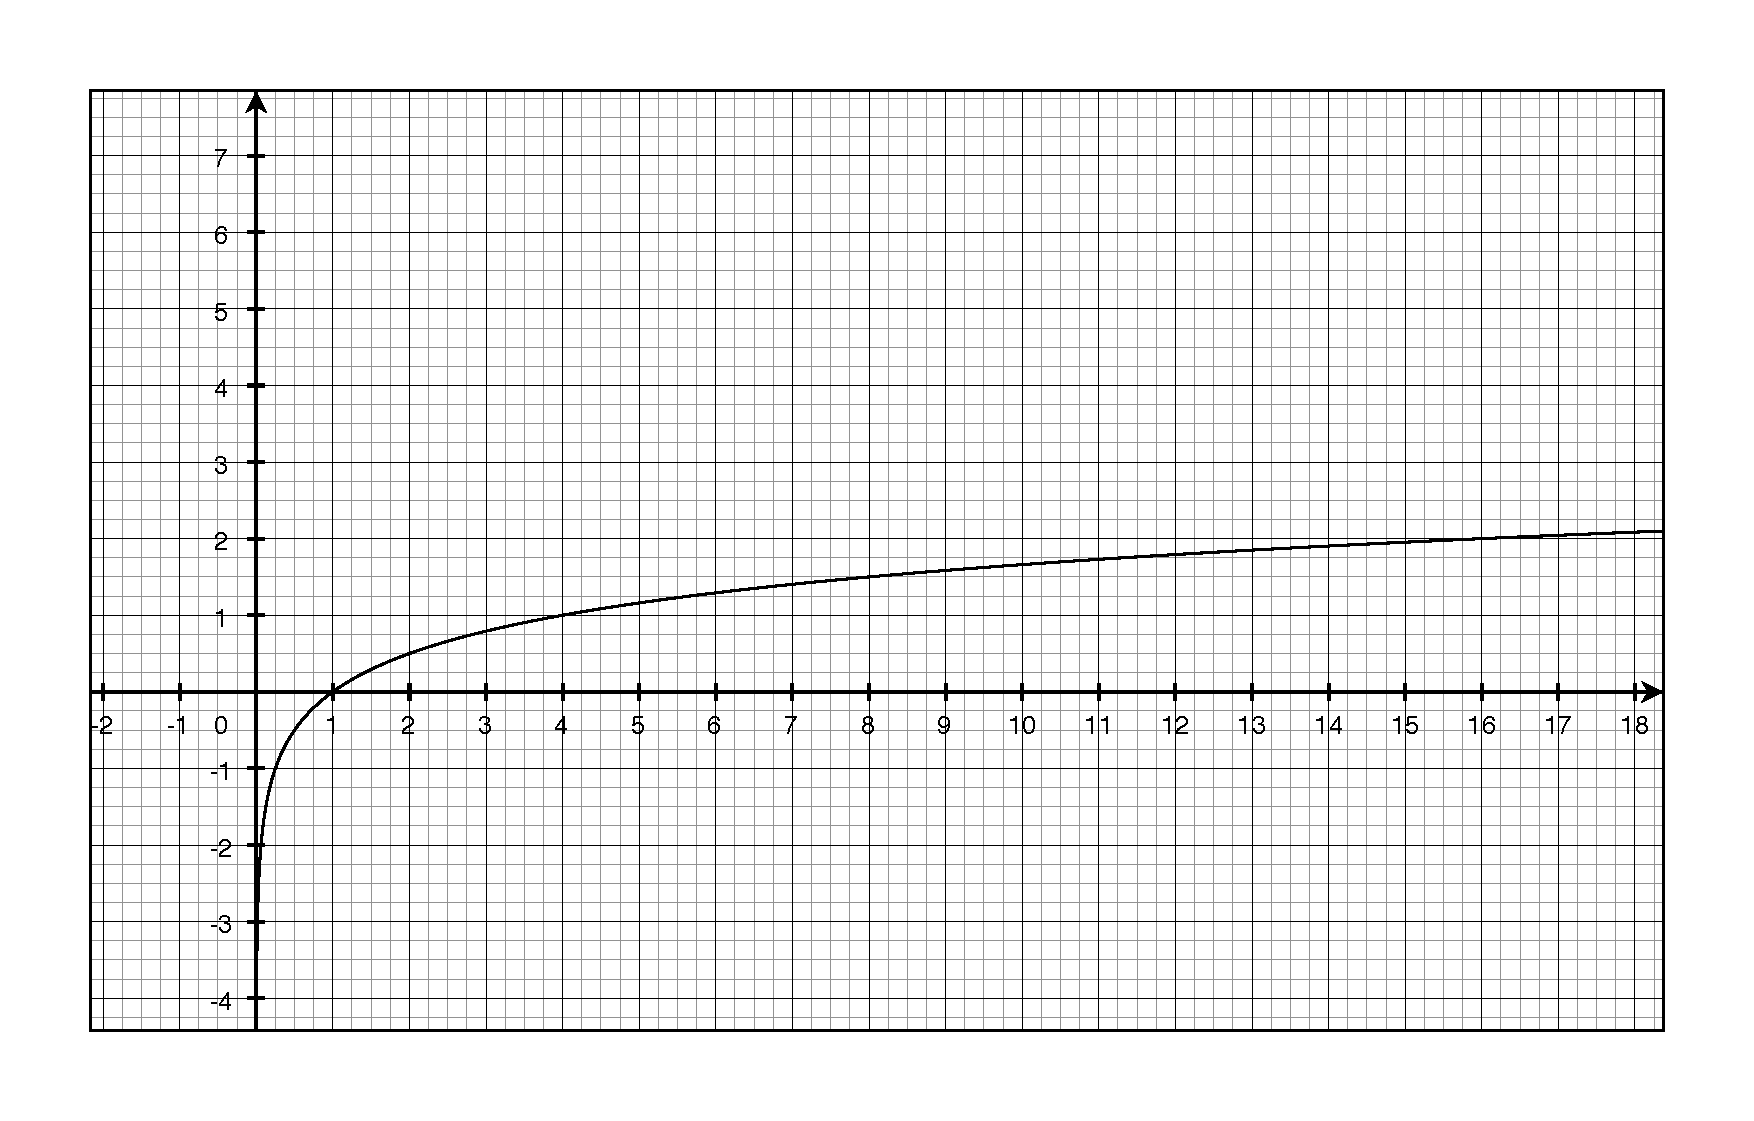
\includegraphics[scale=.3]{question51.eps}
  \caption*{Question 51: $f(x) = \log_4 x$}
\end{figure}

\item[54]

\begin{itemize}
\item domain: $(3, \infty) $
\item x-intercept: $(4, 0) $
\item vertical asymptote: $x = 3$
\end{itemize}

\begin{figure}[H]
  \centering
  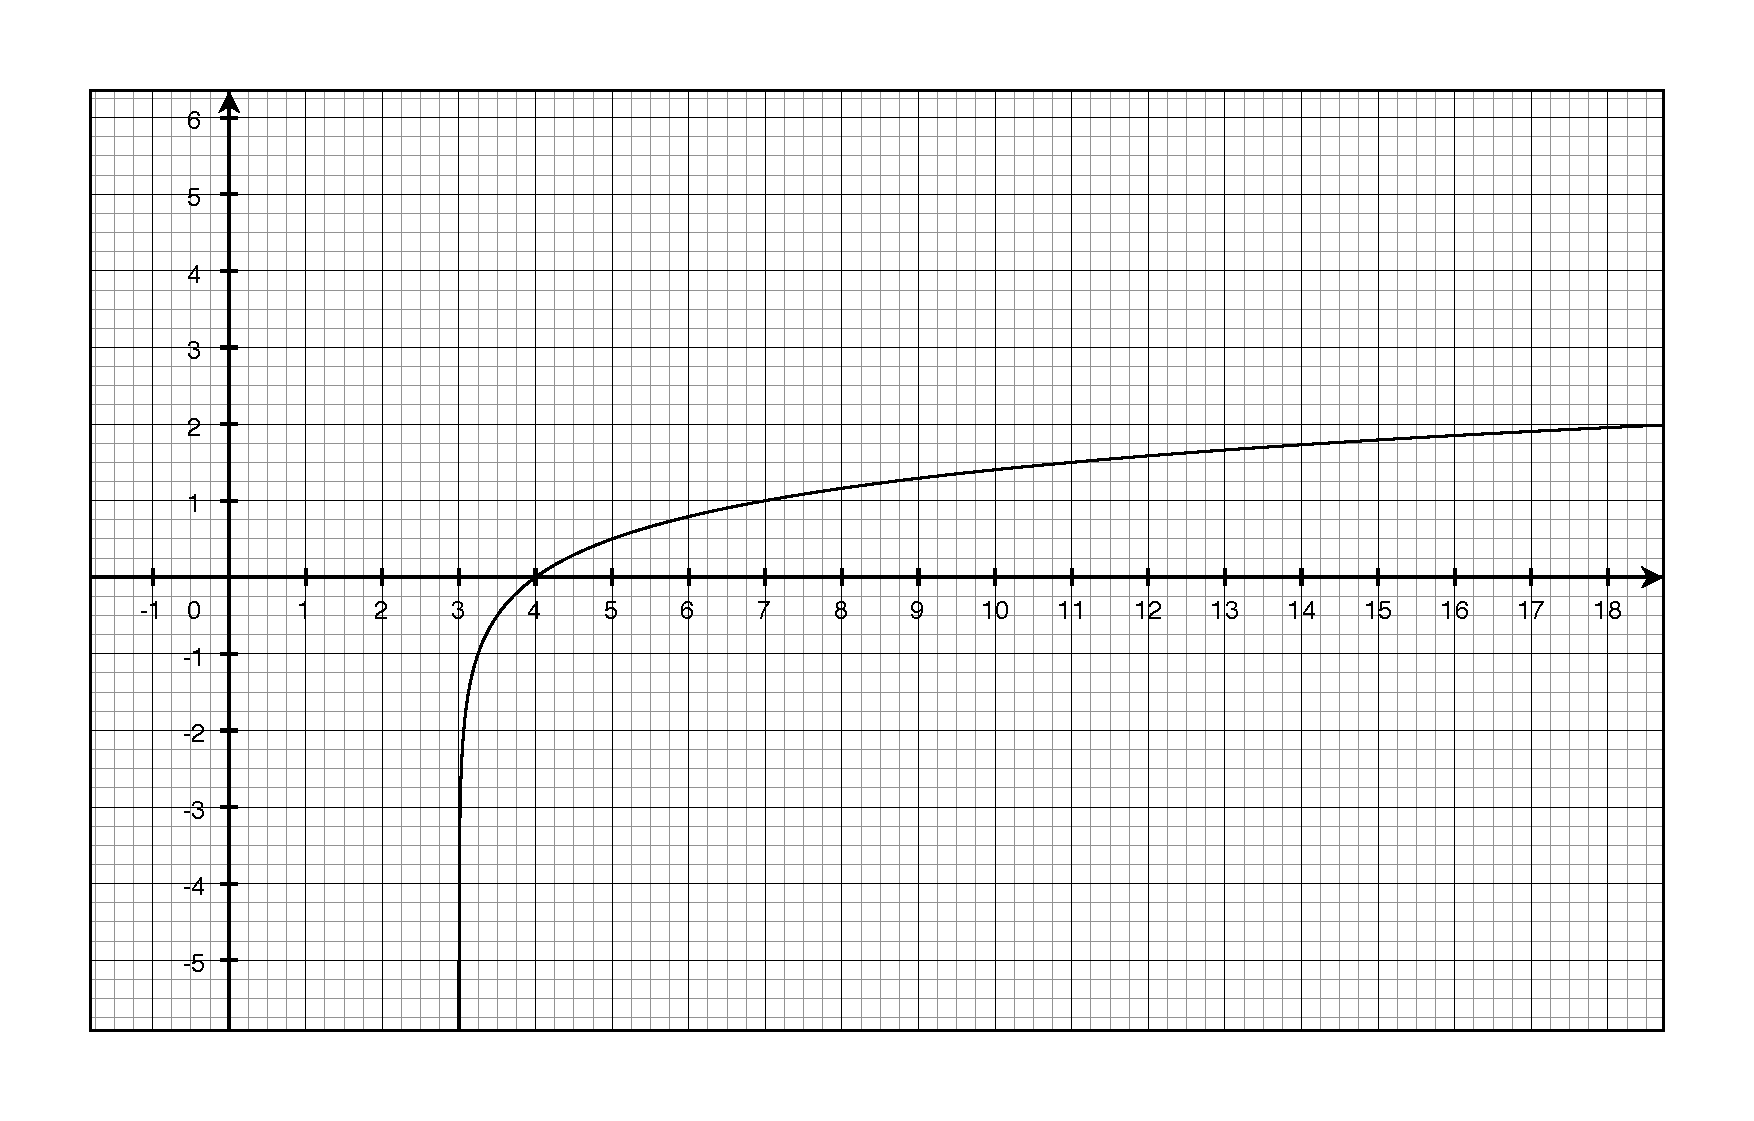
\includegraphics[scale=.3]{question54.eps}
  \caption*{Question 51: $f(x) = \log_4(x - 3)$}
\end{figure}

\item[69]

\begin{description}
\item[a] 
\[
  f(0) = 80 - 17 \log_{10}(1) = 80 
\]

\item[b] 
\[
  f(4) = 80 - 17 \log_{10}(4 + 1) = 68
\]

\item[b] 
\[
  f(10) = 80 - 17 \log_{10}(10 + 1) = 62
\]

\end{description}

\item[76]

\[
  f(I) = 10 \log_{10} \left( \frac{I}{10^{-12}} \right)
\]

\begin{description}
\item[a]
\[
  f(1) = 10 \log_{10} \left( \frac{1}{10^{-12}} \right) = 10 \log_{10} 10^{12} = 10 \cdot 12 = 120
\]

\item[2]
\[
  f(10^{-2}) = 10 \log_{10} \left( \frac{10^{-2}}{10^{-12}} \right) = 10 \log_{10} 10^{10} = 10 \cdot 10 = 100
\]

\item[3]
The number of decibels depends on the ratio of the exponent plus 12, not the ratio of the numbers.  In this
case, the exponents, after adjustment are 12 and 10, so the ratio of the decibels is also 12:10.

Another interesting case is doubling the intensity of the sound.  For example, if we double the intensity of the sound
from part b, we get:

\[
  f(210^{-2}) = 10 \log_{10} \left( \frac{2 \cdot 10^{-2}}{10^{-12}} \right) = 10 \log_{10}(2 \cdot 10^{10}) = 103
\]

Doubling the intensity only gives a 3 dB increase in the sound.


\end{description}

\end{description}

\fi

\ifprintanswers
\else

\vspace{3 in}

{\em The intellectual tradition is one of servility to power, and if I didn't betray it I'd be ashamed of myself.}

\vspace{.1 cm}
\hspace{1 cm} --Noam Chomsky
\fi
\end{document}

